\documentclass[12pt,letterpaper,oneside]{report}

%---------------------PACKAGES
\usepackage[margin=3cm]{geometry}
\usepackage[utf8]{inputenc}
\usepackage{graphicx}
\usepackage[spanish]{babel}
\usepackage[fixlanguage]{babelbib}
\selectbiblanguage{spanish}
\usepackage{url}
\usepackage{float}
%-----------------------------

\title{Trust Me}
\author{{Brayan Arango} \\ {Wilder Alcala}}

%-----------------CONFIG
\renewcommand{\labelitemi}{$\bullet$}
\renewcommand{\labelitemii}{$-$}
\setcounter{tocdepth}{4}
\setcounter{secnumdepth}{4}
%-----------------------

\begin{document}
	
	%-----------------INDEX
	\begin{titlepage}
	\begin{center}
	\textbf{DISEÑO DE UN PROTOTIPO DE PLATAFORMA WEB, QUE PERMITA LA GESTIÓN DE MICROCRÉDITOS ENTRE SUS USUARIOS.}\\
	\vspace{5cm}
	
	{WILDER MANUEL ALCALÁ VIZCAINO}\\
	{BRAYAN CAMILO ARANGO RIVERA}\\ 
	\vspace{4cm}
	
	\includegraphics[width=0.4\textwidth]{start/Universidad}\\
	\vspace{0.5cm}
	
	{UNIVERSIDAD DISTRITAL FRANCISCO JOSÉ DE CALDAS}\\
	{FACULTAD DE INGENIERÍA}\\
	{ESPECIALIZACIÓN EN INGENIERÍA DE SOFTWARE}\\
	{BOGOTÁ D.C, COLOMBIA}\\
	{2019}\\
	\end{center}
\end{titlepage}
	\begin{titlepage}
	\begin{center}
	\textbf{DISEÑO DE UN PROTOTIPO DE PLATAFORMA WEB, QUE PERMITA LA GESTIÓN DE MICROCRÉDITOS ENTRE SUS USUARIOS.}\\
	\vspace{2.5cm}
	
	\textbf{AUTORES:}\\
	{WILDER MANUEL ALCALÁ VIZCAINO}\\
	{BRAYAN CAMILO ARANGO RIVERA}\\ 
	\vspace{2.5cm}
	
	{PROYECTO DE GRADO PRESENTADO PARA OPTAR POR EL TÍTULO DE ESPECIALISTA EN INGENIERÍA DE SOFTWARE.}\\
	\vspace{2.5cm}
	
	\textbf{DIRECTOR:}\\
	{JULIO BARON VELANDIA}\\
	\vspace{1cm}
	
	\textbf{REVISOR:}\\
	{ALEJANDRO PAOLO DAZA CORREDOR}\\
	\vspace{2cm}
	

	
	
	{UNIVERSIDAD DISTRITAL FRANCISCO JOSÉ DE CALDAS}\\
	{FACULTAD DE INGENIERÍA}\\
	{ESPECIALIZACIÓN EN INGENIERÍA DE SOFTWARE}\\
	{BOGOTÁ D.C, COLOMBIA}\\
	{2019}\\
	\end{center}
\end{titlepage}

	\pagenumbering{Roman}
	\urlstyle{same}
	\begin{flushright}
	\textbf{Nota de aceptación}\\
	\vspace{1cm}
	
	\rule{5cm}{0.1mm}\\
	\rule{5cm}{0.1mm}\\
	\rule{5cm}{0.1mm}\\
	\rule{5cm}{0.1mm}\\
	\rule{5cm}{0.1mm}\\
	\rule{5cm}{0.1mm}\\
	\rule{5cm}{0.1mm}\\
	\vspace{3cm}
	
	
	\rule{5cm}{0.1mm}\\
	\textbf{Decano}\\
	\vspace{2.5cm}
	
	\rule{5cm}{0.1mm}\\
	\textbf{Director}\\
	\vspace{2.5cm}
	
	\rule{5cm}{0.1mm}\\
	\textbf{Revisor}\\
	\vspace{2.5cm}
	
	\flushleft \textbf{ Bogotá, D.C 2019}
	
\end{flushright}
	\chapter*{\flushright Dedicatoria}

\begin{flushright}
	\textit{Dedicado a nuestras familias, las cuales han sacrificado \\ su tiempo de compartir con nosotros, por nuestro saber.}
\end{flushright}
	
	%--------------------TABLES
	\tableofcontents
	\listoffigures
	%\listoftables
	
	%-----------------CONTENT
	\addcontentsline{toc}{part}{INTRODUCCION}
\pagenumbering{arabic}
\chapter*{INTRODUCCION}

\textit{Dedicado a nuestras familias, las cuales han sacrificado tiempo para compartir con nosotros, por nuestro saber.}
	
	\part{CONTEXTUALIZACIÓN DE LA INVESTIGACIÓN}
	
		\chapter{DESCRIPCION DE LA INVESTIGACIÓN}
			\section{Estudio del problema de investigación}

	\subsection{Planteamiento del Problema}
	
	{Las entidades bancarias en Colombia, son los entes principales en gestionar créditos para sus clientes, estas se encargan de ofrecer créditos según el perfil de la persona interesada, tomando en cuenta, sus ingresos, la capacidad de endeudamiento y los reportes en las centrales de riesgo, limitando así, el acceso de personas con ingresos bajos y sin vida crediticia, a este tipo de beneficio \cite{bankrep}. Incluso, en algunos casos, el monto del crédito requerido por el usuario es tan bajo, que no amerita el tramite necesario para acceder a él, obligando a la persona a afrontar necesidades básicas las cuales no puede suplir en el momento.\\
		
	A esto se le suma, el aumento de la tasa desempleo que para este año según cifras DANE va en un 10,8\%, aumentando un 1,6\% con respecto al año pasado que estaba en un 9.2\% \cite{dane}, esto gracias, al alto crecimiento de la población \cite{unemployment}, si bien la crisis económica del vecino país Venezuela, ha obligado a gran parte de sus habitantes a migrar hacia Colombia, estos por la falta de empleo y necesidad,  ofrecen sus servicios profesionales a menores rangos salariales,  influyendo en la estabilidad y el bolsillo de los colombianos.\\
	
	Frente a esta problemática y las necesidades expuestas, un grupo de personas que trabajan en la informalidad, como vendedores ambulantes e incluso tenderos, buscando subsanar el alto índice de intereses cobrado por las entidades bancarias, ofrecen sus productos a clientes de confianza con módicas cuotas de pago, facilitándoles el acceso a recursos básicos de bajo costo, los cuales, una entidad financiera normalmente no financiaría, dicho procedimiento es conocido como “fiar”, en otros términos, ofrecer un microcrédito, donde el tendero usualmente toma registro de cada ítem fiado en una agenda o cuaderno, permitiendo fácilmente la manipulación, ingreso errado (malos cálculos) y la perdida, de la información, pues el registro estará supeditado al tendero, conllevando a un alto grado de incertidumbre en el cliente representado en molestar.\\

	Por otro lado, también existe una problemática relacionada en cuanto a préstamos entre conocidos se refiere, pues algunas personas son amantes de las apuestas y a veces se ven envueltos en deudas con sus conocidos por estas, o por causas de fuerza mayor que los obligan a pedir un préstamo de dinero, y es allí donde se presenta la falencia, pues al ser un proceso irrelevante para ellos (por ser de confianza), no toman registro de la transacción o hacen una simple anotación en cuadernos, celulares, agendas etc, permitiendo que la transacción quede en el olvido o se pierda.}

	\subsection{Formulación del problema}
	
	{Con base a la problemática anterior expuesta, surge la siguiente pregunta de investigación ¿Cómo facilitar la gestión de microcréditos entre el tendero, consumidor o personas naturales por medio de una plataforma WEB?.}
	
	\subsection{Sistematización del problema}
	
	\begin{itemize}
		\item ¿Bajo qué fórmulas se rigen las entidades financieras para el cálculo de cuotas, en caso de un usuario pagar a plazos?.
		\item ¿Cómo permitir el fácil acceso a la información de los microcréditos obtenidos por él consumidor, ante él tendero?.
		\item ¿Cómo conservar indefinidamente la información de los microcréditos, sin que esta se pierda por manipulación del usuario?.
	\end{itemize}

			\section{Objetivos}
	\subsection{Objetivo general}
	
	{Desarrollar un prototipo de plataforma WEB, que permita la gestión de microcréditos entre sus usuarios, con el fin de facilitar el cálculo y visualización de estos en una interfaz amigable.}
	
	\subsection{Objetivos específicos}
	
	\begin{itemize}
		\item Aumentar el numero de ventas de los tenderos al basar su sistema de pagos en los microcréditos de la plataforma WEB.
		\item Eliminar la incertidumbre del usuario con respecto a los microcréditos obtenidos.
		\item Reducir el uso desmesurado de microcréditos por parte del usuario, con la limitación de estos, para un mejor manejo de sus finanzas.
	\end{itemize}
	
	
	
	
	
	
			\section{Justificacion}

{En la actualidad, muchas aplicaciones ofrecen servicios de comercio electrónico que satisfacen a la población, con una alta gama de productos y servicios disponibles para la entrega, pero ¿qué pasa cuando estos productos no se pueden conseguir en la ciudad donde los necesitan? Ya sea porque la población de esa ciudad es reacia a consumir estos productos o porque no se fabriquen en dicho lugar. \\
	
Existen otros tipos de empresas que transportan productos entre largos trayectos, pero necesitan de una persona, ya sea familiar o un amigo que lo envié, además de pagar un costo más elevado, que el mismo valor del producto a transportar.  \\

En este sentido, se requiere aportar una solución que baje los costos de traslado y acorte distancias entre personas de la misma región, por eso, es muy importante para un bienestar en la población, facilitar el acceso a esos pequeños elementos que por más pequeños que sean, te hacen sentir como en casa. \\

La presente investigación pretende crear un sistema de comunicación entre las personas para transportar suvenires de manera rápida y a bajos costos, esta, busca ayudar a toda la población que requiera de un producto al que no tengan acceso y, a la población que viaja constantemente y necesite ingresos extras. }
			\section{Alcances y limitaciones}

	\subsection{Alcances}
	\begin{itemize}
		
		\item El desarrollo de la plataforma Web, será un prototipo regido bajo un ambiente controlado de pruebas que proveerá el mini factibilidad del producto.
		\item El cálculo de los pagos que deben realizar los usuarios, estará basado en las fórmulas de cuotas fijas utilizadas en las entidades financieras, todo esto con el fin de garantizar un sistema confiable y sin margen de error.
		
	\end{itemize}
	
	\subsection{Limitaciones}
	\begin{itemize}
		
		\item La plataforma web sólo brindará soporte en escritorio y no nativamente en móvil, ya que no se posee el conocimiento adecuado para este tipo de desarrollo.
		
		\item Inicialmente la plataforma solo permitirá el pago en efectivo (emulando el método de pago de las personas que usualmente fían), no tendrá un pago digital, debido a los costos adicionales que acarrearía el proyecto por este tipo de pago.
		
	\end{itemize}
			\section{Hipótesis}

{Dado los avances tecnológicos y el gran acogimiento que este ha tenido en la actualidad, el desarrollo de una plataforma web que permita la gestión de microcréditos entre sus usuarios, facilitara el acceso a recursos de baja demonimacion, con pagos a cuotas y aumentara las ventas de quienes la utilicen.}
			\section{Marco referencial}

	\subsection{Marco teórico}
	
		\subsubsection{Microcrédito}
		
		{Es una fuente de financiación enfocada a los hogares con bajos ingresos, esta, trata de proveer pequeños prestamos impulsando el desarrollo económico de los interesados, permitiendo la adquisición de activos o bienes de bajo costo, es basada en la hipótesis de "para bajar los índices de pobreza es indispensable dar acceso a los recursos financieros" \cite{MaricruzMicro,BarbaraMicro}.\\
		
		El microcrédito, es imprecindible como fuente de financiación para las personas que se encargan a las ventas informales, este permite que sus clientes tengan acceso a sus productos, incrementar el porcentaje de sus ventas y fidelizar a los mismos \cite{LupeTrust}.\\
	
		\begin{figure}[H]
			\centering
			\includegraphics[width=0.8\linewidth]{description/framework/tendero.jpg}
			\caption{Tendero fiando}
		\end{figure}
		}
	
	
		\subsubsection{Experiencia de usuario}
		
		{La experiencia de usuario hace referencia a la visión o al diseño en la que el proceso o interactividad de la aplicación, está delimitada o conducida empíricamente por la información recopilada de la audiencia objetivo del producto, esto con el fin de garantizar una navegabilidad fluida entre cada uno de sus usuarios, para esto, es necesario tener en cuenta la “interacción”, previsualizando las opciones de las que dispondrá el usuario y como deberá responder la aplicación a cada una de sus acciones \cite{YusefUX}.\\
		
		La interacción, es divisible en 3 etapas:
		
		\begin{itemize}
			\item \textbf{Formulación del objetivo:} ¿Que quiere lograr el usuario?
			\item \textbf{Ejecución:} ¿Qué hace?
			\item \textbf{Evaluación:} El usuario compara lo que ocurrió, con que quería que ocurriera.
		\end{itemize}
		
		\begin{figure}[H]
			\centering
			\includegraphics[width=0.8\linewidth]{description/framework/interactividad.jpg}
			\caption{Interactividad}
		\end{figure}
		}
	
		\subsubsection{Almacenamiento y persistencia de la información}
		
		{Los desarrollos tecnológicos en la informática y en la electrónica, han permitido que el almacenamiento de la información, pase de ser físico a digital, utilizando herramientas de almacenamiento en la nube para su posterior uso, conocidos como bases de datos, esto, facilitando la obtención de datos inmediatamente cuando son requeridos y garantizando el acceso a ellos.\\
			
		Las bases de datos, son un conjunto de datos almacenados en un medio informático que puede ser accedido por varios usuarios o aplicaciones a la vez, teniendo en cuenta como premisa, que estos no pueden ser redundantes e innecesarios.  \cite{angelData}.\\
		
		\begin{figure}[H]
			\centering
			\includegraphics[width=0.8\linewidth]{description/framework/nube.jpg}
			\caption{Almacenamiento en la nube}
		\end{figure}
	}
		
	
	\subsection{Marco Conceptual}
	
		\subsubsection{Sitios Web}
		
		{Un sitio web es un conjunto de archivos electrónicos y páginas web referentes a un tema en particular, incluyendo una página inicial de bienvenida generalmente denominada home page, a los cuales se puede acceder a través de un nombre de dominio y dirección en Internet específicos. El World Wide Web, o simplemente Web como se le llama comúnmente, está integrado por sitios web y éstos a su vez por páginas web. La gente suele confundir estos términos, pero un sitio web es en realidad un conjunto de páginas web.\\
			
		Los sitios web son empleados por las instituciones públicas y privadas, organizaciones e individuos para comunicarse con el mundo entero. En el caso particular de las empresas, este mensaje tiene que ver con la oferta de sus bienes y servicios a través de Internet, y en general para hacer eficiente sus funciones de mercadotecnia.}
		
		
		\subsubsection{Diseño Web responsivo}
		
		{El diseño web responsive o adaptativo es una técnica de diseño web que busca la correcta visualización de una misma página en distintos dispositivos. Desde ordenadores de escritorio a tablets y móviles, en otras palabras, se trata de redimensionar y colocar los elementos de la web de forma que se adapten al ancho de cada dispositivo permitiendo una correcta visualización y una mejor experiencia de usuario. Se caracteriza porque los layouts (contenidos) e imágenes son fluidos y se usa código media-queries de CSS3.\\
			
		El diseño responsive permite reducir el tiempo de desarrollo, evita los contenidos duplicados, y aumenta la viralidad de los contenidos ya que permite compartirlos de una forma mucho más rápida y natural.}
	
		
		\subsubsection{Bases de datos relaciones}
		
		{Una base de datos relacional consiste en un conjunto de tablas, a cada una de las cuales se le asigna un nombre exclusivo, cada fila de la tabla representa una relación entre un conjunto de valores. De manera informal, cada tabla es un conjunto de entidades, y cada fila es una entidad, dado que cada tabla es un conjunto de tales relaciones, hay una fuerte correspondencia entre el concepto de tabla y el concepto matemático de relación, del que toma su nombre el modelo de datos relacional.}
	
		\subsubsection{SQL}
		
		{El álgebra relacional proporciona una notación concisa y formal para la representación de las consultas. Sin embargo, los sistemas de bases de datos comerciales necesitan un lenguaje de consultas más cómodo para el usuario. SQL es un lenguaje de consultas distribuido comercialmente de más influencia. SQL usa una combinación de constructores del álgebra relacional y del cálculo relacional.\\
			
		Aunque se haga referencia al lenguaje SQL como “lenguaje de consultas”, puede hacer mucho más que consultar las bases de datos. Usando SQL es posible además definir la estructura de los datos, modificar los datos de la base de datos y especificar restricciones de seguridad.\\
	
		No se pretende proporcionar un manual de usuario completo de SQL. En cambio, se presentan los constructores y conceptos fundamentales de SQL. Las distintas implementaciones de SQL pueden diferenciarse en detalles o admitir sólo un subconjunto del lenguaje completo.}
	
	
		\subsubsection{RESTful}
		
		{La Transferencia de Estado Representacional (REST - Representational State Transfer) fue ganando amplia adopción en toda la web como una alternativa más simple a SOAP y a los servicios web basados en el lenguaje de descripción de servicios Web (Web Services Descripcion Language - WSDL). Ya varios grandes proveedores de Web 2.0 están migrando a esta tecnología, incluyendo a Yahoo, Google y Facebook, quienes marcaron como obsoletos a sus servicios SOAP y WSDL y pasaron a usar un modelo más fácil de usar, orientado a los recursos.\\
			
		REST define un set de principios arquitectónicos por los cuales se diseñan servicios web haciendo foco en los recursos del sistema, incluyendo cómo se accede al estado de dichos recursos y cómo se transfieren por HTTP hacia clientes escritos en diversos lenguajes. REST emergió en los últimos años como el modelo predominante para el diseño de servicios. De hecho, REST logró un impacto tan grande en la web que prácticamente logró desplazar a SOAP y las interfaces basadas en WSDL por tener un estilo bastante más simple de usar.}
	
	
		\subsubsection{Web API}
		
		{Es un marco que facilita la creación de servicios HTTP disponibles para una amplia variedad de clientes, entre los que se incluyen exploradores y dispositivos móviles. ASP.NET Web API es la plataforma perfecta para crear aplicaciones RESTful en .NET Framework.}
		
		
		\subsubsection{HTTP}
		
		{Hypertext Transfer Protocol (HTTP) (o Protocolo de Transferencia de Hipertexto en español) es un protocolo de la capa de aplicación para la transmisión de documentos hipermedia, como HTML. Fue diseñado para la comunicación entre los navegadores y servidores web, aunque puede ser utilizado para otros propósitos también. Sigue el clásico modelo cliente-servidor, en el que un cliente establece una conexión, realizando una petición a un servidor y espera una respuesta del mismo. Se trata de un protocolo sin estado, lo que significa que el servidor no guarda ningún dato (estado) entre dos peticiones. Aunque en la mayoría de casos se basa en una conexión del tipo TCP/IP, puede ser usado sobre cualquier capa de transporte segura o de confianza, es decir, sobre cualquier protocolo que no pierda mensajes silenciosamente, tal como UDP.}
		
		
		\subsubsection{Modelo Cliente - Servidor}
		
		{Modelo de diseño de software en el que las tareas se reparten entre los proveedores de recursos o servicios, llamados servidores, y los demandantes, llamados clientes. Un cliente realiza peticiones a otro programa, el servidor, quien le da respuesta.}
	
	
		\subsubsection{Arquitectura Orientada a Servicios SOA}
		
		{Modelo de diseño de software en el que las tareas se reparten entre los proveedores de recursos o servicios, llamados servidores, y los demandantes, llamados clientes. Un cliente realiza peticiones a otro programa, el servidor, quien le da respuesta.}
			\section{Aspectos metodológicos}

	\subsection{Tipo de estudio}
	
	{Dado el tema de investigación, el tipo de estudio a realizar se enmarca dentro del tipo descriptivo, el cual, pretende dar una descripción del objeto de estudio, especificando sus propiedades o atributos más relevantes, para así, fortalecer la justificación del porqué el desarrollo del proyecto \cite{methoInv}, se acudirá a la implementación de técnicas de recolección de información, basadas en la observación, entrevistas y/o cuestionarios, permitiendo la identificación de la tendencia actualmente de las personas, por utilizar plastaformas para alcanzar o conseguir un bien común, tal como se evidencia en plataformas populares como uber, uber eats, rappi, etc.}
	
	
	\subsection{Método de investigación}
	
	{El método a implementar en este estudio investigativo, es el de la observación, el cual, permitirá obtener conocimiento acerca del fenómeno presentado actualmente dentro de las comunidades que emplean medios tecnológicos, se enfoca en observar para obtener información del problema, estimulando la curiosidad e impulsando al desarrollo de nuevos hechos de interés científico, es ideal, para el tipo de estudio planteado, ya que se puede complementar con la utilización de otros procedimientos o técnicas propuestos, como lo son entrevistas y cuestionarios, permitiendo la comparación de los resultados recogidos y obtener una información más precisa, haciendo posible investigar el fenómeno tecnológico directamente \cite{methoInv,metho}.}
	
	
	\subsection{Fuentes y técnicas para la recolección de la información}
	
	{Para la recolección de información nos basaremos en las fuentes primarias, las cuales, serían los usuarios de tecnologías orientadas a comunidades, como usuarios de Uber, rappi, etc, de ellos, obtendremos la información directa por medio de las técnicas antes mencionadas:
		
	\begin{itemize}
		\item \textbf{Encuestas:} se realiza el registro de situaciones que puedan ser observadas y en ausencia de poder ser recreado un experimento se cuestiona al participante sobre ello.
		
		\item \textbf{Experimentación:} Se manipulan las variables que rodean la problemática, permitiendo analizar los efectos causados por estos y verificar si las diferencias obtenidas son significativas.
	\end{itemize}
		
	Adicionalmente, se obtendrá información de fuentes secundarias como lo son documentos de internet o medios de comunicación, siempre y cuando, la información sea pertinente y fidedigna \cite{learn}.}
	
	\subsection{Tratamiento de la información}
	
	{Se realizará un análisis cualitativo de la información obtenida, realizando una conversión de esta y garantizando una mirada crítica para filtrar la información que constituirá la fuente principal de la investigación, desligando de datos complementarios, que también serán útiles para el desarrollo del proyecto \cite{methoqual}.}
			
	\part{DESARROLLO DE LA INVESTIGACIÓN}
		
		\chapter{METODOLOGÍA APLICADA}
			\section{Metodología ágil SCRUM}

{Tal y como lo explica la guía de Scrum, es un marco de trabajo, un framework por el cual las personas pueden abordar problemas complejos adaptativos, a la vez que entregan productos del máximo valor posible de forma productiva y creativa, scrum se basa en la teoría de control de procesos empírica o empirismo, que asegura que el conocimiento procede de la experiencia y de tomar decisiones basándose en lo que se conoce.\\

El plan del sprint es creado por todos los miembros del equipo Scrum de forma colaborativa. En esta ceremonia se toman todas las historias de usuario priorizadas y se decide sobre cuáles hacer el Sprint tomando como base el objetivo del sprint y la capacidad del equipo. Se define qué puede entregarse en el Incremento resultante del Sprint que comienza y cómo se conseguirá hacer el trabajo necesario para entregar el Incremento. Si bien Scrum no establece un método para estimar es recomendable utilizar alguno como, por ejemplo, la estimación en puntos de historia para cada uno de los elementos del sprint backlog.

	\subsection{Personas y roles del Proyecto}
	{\begin{figure}[H]
		\centering
		\includegraphics[width=1\linewidth]{development/roles.png}
		\caption{Roles y actores}
	\end{figure}}
	\begin{center}
		\textbf{Fuente:} Propia.
	\end{center}
	\hfill

	\subsection{Pila del Sprint}
	{En esta sección se describe de forma detallada los requisitos o tareas que va a desarrollar el equipo de trabajo en cada iteración.
	
		\subsubsection{Responsabilidades del gestor de producto}
		{Presencia en las reuniones en las que el equipo elabora la pila del sprint. Resolución de dudas sobre las historias de usuario que se descomponen en la pila del sprint}
		
		\subsubsection{Responsabilidades del equipo técnico}
			\begin{itemize}
				\item Elaboración de la pila del sprint.
				\item Resolución de dudas o comunicación de sugerencias sobre las historias de usuario con el gestor del producto.
			\end{itemize}
	}

	\subsection{Pila del Producto}
	{A continuación, se define la lista de requisitos o requerimientos funcionales que debe cumplir el sistema de acuerdo a la solicitud del cliente.
		
	El requisito principal del proyecto es crear un prototipo que permita la gestión de micro transacciones entre sus usuarios.\\
		
		\begin{itemize}
			\item \textbf{Modulo administrador:} permite la gestión de usuarios administrando los permisos, menús etc. según cada uno de los perfiles asignados.
			\item \textbf{Registrar préstamo:} Permitir el registro del préstamo de una forma intuitiva.
			\item \textbf{Obtener préstamo:} Permitir a través de un código QR, asignarse un préstamo.
			\item \textbf{Pagar préstamo y aceptar pagos:} Movimientos realizados al préstamo.
		\end{itemize}
	
	}

	\subsection{Primera Iteración}
	{La primera fase del proyecto será desarrollar las actividades referentes a la parte administrativa donde se van a gestionar los permisos, perfiles y menús del prototipo.\\
	
	\begin{figure}[H]
			\centering
			\includegraphics[width=1\linewidth]{development/sprint1.png}
			\caption{Sprint 1}
	\end{figure}
	\begin{center}
		\textbf{Fuente:} Propia.
	\end{center}

	\begin{itemize}
		
		\item \textbf{Incremento:} Luego de asignar las tareas relacionadas con el módulo de administración de usuarios del proyecto se obtiene el primer incremento, el cual consiste de todos los CRUD con los cuales es posible otorgar permisos a los usuarios y perfiles.
			
		
		\item Listar menús
			\begin{figure}[H]
				\centering
				\includegraphics[width=1\linewidth]{development/listarmenu.png}
				\caption{Lista de menus - Tru\$tMe}
			\end{figure}
			\begin{center}
				\textbf{Fuente:} Propia.
			\end{center}
			\hfill \break
		
		\item Crear menús
		\begin{figure}[H]
			\centering
			\includegraphics[width=1\linewidth]{development/crearmenu.png}
			\caption{Creación de menus - Tru\$tMe}
		\end{figure}
		\begin{center}
			\textbf{Fuente:} Propia.
		\end{center}
	
		\item Actualizar menú
		\begin{figure}[H]
			\centering
			\includegraphics[width=1\linewidth]{development/actualizarmenu.png}
			\caption{Actualización de menus - Tru\$tMe}
		\end{figure}
		\begin{center}
			\textbf{Fuente:} Propia.
		\end{center}
		
		\item Listar perfiles
		\begin{figure}[H]
			\centering
			\includegraphics[width=1\linewidth]{development/listarperfiles.png}
			\caption{Listar perfiles - Tru\$tMe}
		\end{figure}
		\begin{center}
			\textbf{Fuente:} Propia.
		\end{center}
		\hfill
		
		\item Crear perfiles
		\begin{figure}[H]
			\centering
			\includegraphics[width=1\linewidth]{development/crearperfiles.png}
			\caption{Creación de perfiles - Tru\$tMe}
		\end{figure}
		\begin{center}
			\textbf{Fuente:} Propia.
		\end{center}
		\hfill \break
		\hfill \break
		\hfill \break
		
		\item Actualizar perfiles
		\begin{figure}[H]
			\centering
			\includegraphics[width=1\linewidth]{development/actualizarperfiles.png}
			\caption{Actualización de perfiles - Tru\$tMe}
		\end{figure}
		\begin{center}
			\textbf{Fuente:} Propia.
		\end{center}
	
		\item Otorgar permisos a un perfil
		\begin{figure}[H]
			\centering
			\includegraphics[width=1\linewidth]{development/otorgarpermisos.png}
			\caption{Otorgació de permisos - Tru\$tMe}
		\end{figure}
		\begin{center}
			\textbf{Fuente:} Propia.
		\end{center}
		
		 
	\end{itemize}
		

		
	}

		\subsection{Segunda Iteración}
		{La segunda fase del proyecto será desarrollar las actividades referentes a la creación del CRUD referente a la creación del préstamo.\\
			
			\begin{figure}[H]
				\centering
				\includegraphics[width=1\linewidth]{development/sprint2.png}
				\caption{Sprint 2}
			\end{figure}
			\begin{center}
				\textbf{Fuente:} Propia.
			\end{center}
			
			\begin{itemize}
				
				\item \textbf{Incremento:} Luego de asignar las tareas relacionadas con el módulo de guardar préstamo se obtiene el segundo incremento, el cual consiste en el formulario de crear préstamo.
				
				
				\item Guardar préstamos
				\begin{figure}[H]
					\centering
					\includegraphics[width=1\linewidth]{development/guardarprestamos.png}
					\caption{Guardar préstamos - Tru\$tMe}
				\end{figure}
				\begin{center}
					\textbf{Fuente:} Propia.
				\end{center}		
					
			\end{itemize}
			
			
			
		}

		\subsection{Tercera Iteración}
		{La tercera fase del proyecto será desarrollar las actividades referentes a la obtención de los préstamos.\\
			
			\begin{figure}[H]
				\centering
				\includegraphics[width=1\linewidth]{development/sprint3.png}
				\caption{Sprint 3}
			\end{figure}
			\begin{center}
				\textbf{Fuente:} Propia.
			\end{center}
				
			\begin{itemize}
				
				\item \textbf{Incremento:} Luego de asignar las tareas relacionadas con el módulo de obtener préstamo se obtiene el tercer incremento, el cual consiste en el formulario para que el prestatario pueda adquirir un préstamo.
				
				
				\item Escanear QR
				\begin{figure}[H]
					\centering
					\includegraphics[width=1\linewidth]{development/escanearqr.png}
					\caption{Escanear QR - Tru\$tMe}
				\end{figure}
				\begin{center}
					\textbf{Fuente:} Propia.
				\end{center}
					
				\item Resumen de préstamos
				\begin{figure}[H]
					\centering
					\includegraphics[width=1\linewidth]{development/resumenprestamos.png}
					\caption{Resumen de préstamos - Tru\$tMe}
				\end{figure}
				\begin{center}
					\textbf{Fuente:} Propia.
				\end{center}
	
				
			\end{itemize}
			
			
			
		}

}
	



			\input{development/cases}
			\section{Diseño interfaz de usuario inicial – wireframe}

{Dada la lógica en los casos de uso, se procede a estructurar la interfaz de usuario y la usabilidad de esta, teniendo en cuenta a los usuarios objetivo, quienes son personas de baja escolaridad y con un bajo dominio de los medios tecnológicos, por tal motivo, la interfaz debe ser sencilla, con pocos botones e intuitiva  nos apoyamos en la guía visual “wireframe” que nos posibilito la creación de un esqueleto o estructura inicial del sitio WEB, dando como resultado lo siguiente:

\begin{figure}[H]
	\centering
	\includegraphics[width=1\linewidth]{development/wireframe.png}
	\caption{Wireframe}
\end{figure}
}
			\section{Diseño base de datos}

{Dada la lógica y el diseño de la interfaz de usuario, se procede a crear la base de datos aplicando las reglas de normalización y así minimizar o evitar la redundancia de datos.

\begin{figure}[H]
	\centering
	\includegraphics[width=1\linewidth]{development/modelo.png}
	\caption{Modelo relacional}
\end{figure}
}
		
		\chapter{ORGANIZACIÓN}
			\section{Introducción}

{En este capítulo se le da un enfoque de negocio al proyecto de grado, se le concede un nombre comercial en inglés “Tru\$tMe”, el cual traducido al español significa confíame, se estable una estructura organizacional que aborda los aspectos empresariales del proyecto.}
			\section{Tru\$tMe}

{Es una empresa colombiana dedica a la gestión de préstamos o “fios” entre sus usuarios, esta permite que la persona que ingrese con un rol de tendero, pueda ofertar sus productos y quienes estén interesados (conocidos del tendero) acceder a los mismos con facilidades de pago, como lo es el pago a cuotas.}
			\section{Misión}

{Ser la empresa líder colombiana en la gestión de préstamos entre sus usuarios, permitiendo el aumento de las ventas de las personas que confíen en la app como herramienta para vender sus productos y brindando transacciones confiables a sus clientes.}
			\section{Visión}

{Influir en la economía de los principales almacenes de cadena de Colombia, como herramienta de gestión de créditos, permitiendo aumentar la clientela objetivo y aportar al crecimiento económico de los colombianos de bajos recursos.}
			\section{Objetivos operativos}

\begin{itemize}
	\item Controlar los préstamos realizados por los tenderos a sus clientes, con la ayuda  de una interfaz amigable.
	\item Brindar acceso a las personas de bajos recursos, a productos de la canasta familiar, con facilidades de pago.
	\item Permitir a las personas naturales prestar dinero a sus conocidos, sin riesgo de perder la información del préstamo.
\end{itemize}
			\section{Principios fundadores}

\begin{itemize}
	
	\item Las entidades colombianas, quienes limitan a las personas de bajos recursos a acceder a una vida digna, con la adquisición de productos de bajo costo que suplan sus necesidades básicas, no están cumpliendo con los principios de igualdad y le están negando el desarrollo económico como persona y ciudadano, a quien lo necesita.
	
	\item Para un mejor desarrollo y sostenibilidad económica, se les debe facilitar el acceso a herramientas tecnológicas, a las personas quienes con tanto esfuerzo han logrado surgir con pequeños negocios, ayudándolos a competir con grandes empresas en igualdad de condiciones.
	
\end{itemize}
			\section{Servicios}

{Los principales servicios que ofrece la aplicación web son los siguientes:

\begin{itemize}
	\item Pagos de deudas.
	\item Pedir préstamos.
	\item Fiar productos.
	\item Ofertar productos.
	\item Calcular pagos.
	\item Calcular intereses.
\end{itemize}
}
			\section{Productos}

{El producto es una plataforma o aplicación WEB capaz de gestionar los préstamos de cada uno de sus usuarios, permitiéndoles avanzar tecnológicamente y abandonar procesos ineficientes de control de finanzas.}
			%\input{development/processes}
			%\input{development/functions}
			
		\chapter{ARQUITECTURA EMPRESARIAL}
			\section{Arquitectura capa de negocio}
{Esta capa, es la capa de arquitectura del proyecto orientada al negocio, aquí se plasma el enfoque organizacional, las reglas que regirán el negocio y las entidades que representan el sistema, permitiendo obtener de forma optima los roles y actores que aquí se desempeñan.}

	\subsection{Punto de vista de organización}
	{ El punto de vista organizacional esta enfocado a la estructura interna de la empresa, departamento o entidad organizacional, este refleja de forma jerárquica el nivel de los actores y roles que aquí interactúan \cite{archimate}.\\
		
		\textbf{Modelo}\\
		\begin{figure}[H]
			\centering
			\includegraphics[width=0.8\linewidth]{development/organizacion.png}
			\caption{Metamodelo de Organización}
		\end{figure}
	
		\textbf{Caso}\\
		
		\begin{figure}[H]
			\centering
			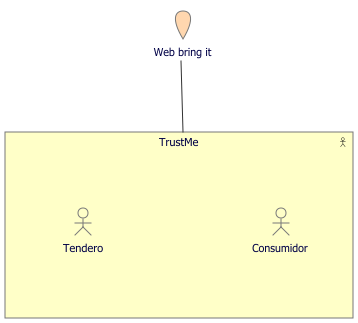
\includegraphics[width=0.8\linewidth]{development/negocio.pdf}
			\caption{Organización}
		\end{figure}
	}
	
	\subsection{Punto de vista de cooperación de actor}
	{ 
		
		\textbf{Modelo}\\
		\begin{figure}[H]
			\centering
			\includegraphics[width=0.8\linewidth]{development/cooperacionactor.png}
			\caption{Metamodelo de cooperación de actor}
		\end{figure}
		
		\textbf{Caso}\\
		
		\begin{figure}[H]
			\centering
			\includegraphics[width=0.8\linewidth]{development/cooperacionactor.pdf}
			\caption{Cooperación de actor}
		\end{figure}
	}
	
	\subsection{Punto de vista de función de negocio}
	{ 
		
		\textbf{Modelo}\\
		\begin{figure}[H]
			\centering
			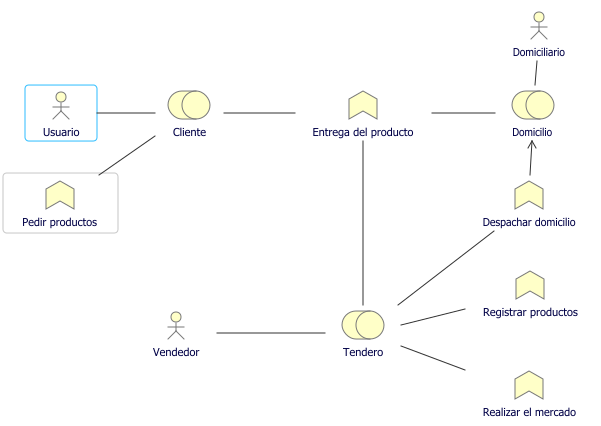
\includegraphics[width=0.8\linewidth]{development/funcion.png}
			\caption{Metamodelo de función de negocio}
		\end{figure}
		
		\textbf{Caso}\\
		
		\begin{figure}[H]
			\centering
			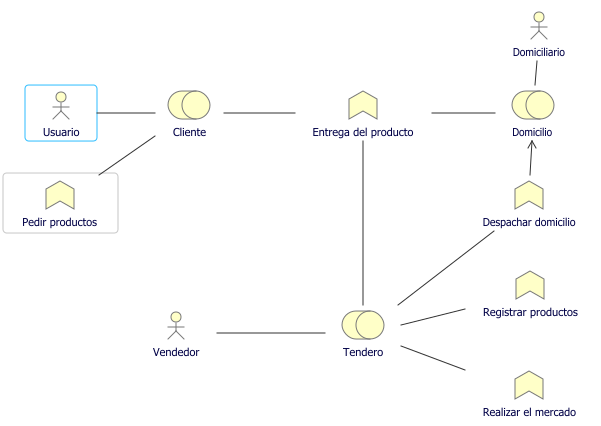
\includegraphics[width=0.8\linewidth]{development/funcion.pdf}
			\caption{Función de negocio}
		\end{figure}
	}
	
	\subsection{Punto de vista de proceso de negocio}
	{ 
		
		\textbf{Modelo}\\
		\begin{figure}[H]
			\centering
			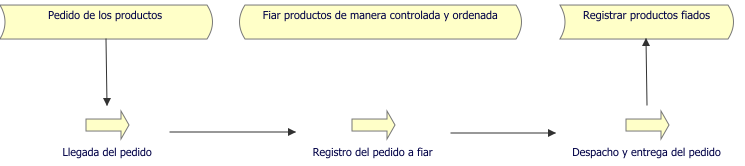
\includegraphics[width=0.8\linewidth]{development/proceso.png}
			\caption{Metamodelo de proceso de negocio}
		\end{figure}
		
		\textbf{Caso}\\
		
		\begin{figure}[H]
			\centering
			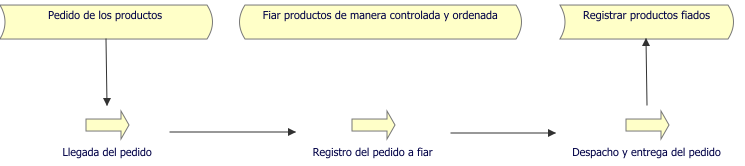
\includegraphics[width=0.8\linewidth]{development/proceso.pdf}
			\caption{Proceso de negocio}
		\end{figure}
	}
	
	\subsection{Cooperación de proceso de negocio}
	{ 
		
		\textbf{Modelo}\\
		\begin{figure}[H]
			\centering
			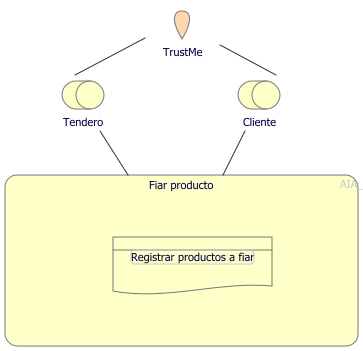
\includegraphics[width=0.8\linewidth]{development/cooperacionproceso.png}
			\caption{Metamodelo de cooperación de proceso de negocio}
		\end{figure}
		
		\textbf{Caso}\\
		
		
		\begin{figure}[H]
			\centering
			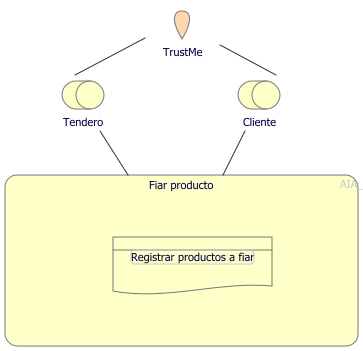
\includegraphics[width=0.8\linewidth]{development/cooperacionproceso.pdf}
			\caption{Cooperación de proceso de negocio}
		\end{figure}
	}
	
	\subsection{Punto de vista de producto}
	{
		
		\textbf{Modelo}\\
		\begin{figure}[H]
			\centering
			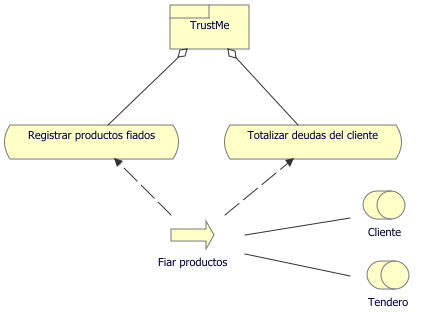
\includegraphics[width=0.8\linewidth]{development/producto.png}
			\caption{Metamodelo de producto}
		\end{figure}
		
		\textbf{Caso}\\
	
		
		\begin{figure}[H]
			\centering
			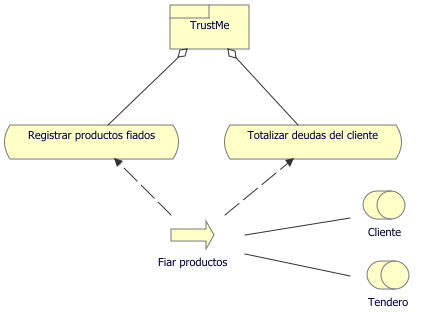
\includegraphics[width=0.8\linewidth]{development/producto.pdf}
			\caption{Producto}
		\end{figure}
	}
			\section{Arquitectura capa de aplicación}
{Esta capa, es la capa de arquitectura del proyecto orientada al aplicación, aquí se plasma la estructura de la aplicación del software soportado en componentes reusables e interfaces de comunicación \cite{archimate}.}

	\subsection{Punto de vista de comportamiento de aplicación}
	{ El comportamiento de aplicación muestra cómo se componen internamente una aplicación, es útil para diseñar el comportamiento principal del sistema o componentes, e identificar la superposición funcional de estas \cite{archimate}.\\
	\newpage
		
		\textbf{Modelo}\\
		\begin{figure}[H]
			\centering
			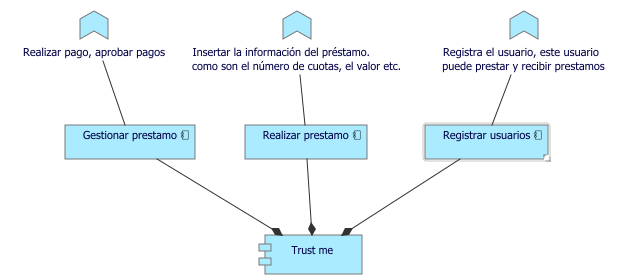
\includegraphics[width=0.8\linewidth]{development/comportamientoapp.png}
			\caption{Metamodelo Comportamiento de Aplicación}
		\end{figure}
		\begin{center}
			\textbf{Fuente:} Colosoft E.U: Documento CasoColoSoft.
		\end{center}
		\hfill \break
			
		\textbf{Caso:} Los componentes de aplicación son:
		
		\begin{itemize}
			\item Gestionar préstamo
			\item Realizar préstamo
			\item Registrar usuarios
		\end{itemize}
		
		\begin{figure}[H]
			\centering
			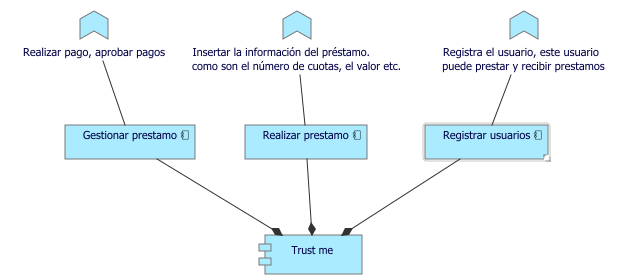
\includegraphics[width=0.6\linewidth]{development/comportamientoapp.pdf}
			\caption{Comportamiento de Aplicación}
		\end{figure}
		\begin{center}
			\textbf{Fuente:} Propia.
		\end{center}
	}
	
	\subsection{Punto de vista de cooperación de aplicación}
	{La  cooperación de aplicación describe las relaciones entre los componentes en términos de flujo de información o en términos de los servicios que estos proveen o usan. Este punto de vista también es usado para expresar la cooperación interna u orquestación de servicios que juntos soportan la ejecución de un proceso de negocio \cite{archimate}.\\
		
		\textbf{Modelo}\\
		\begin{figure}[H]
			\centering
			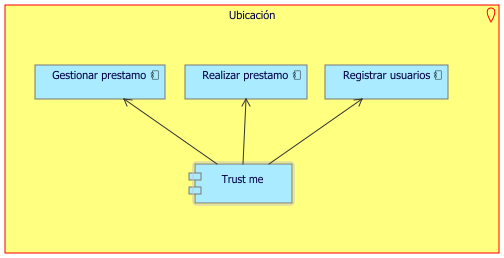
\includegraphics[width=0.8\linewidth]{development/cooperacionapp.png}
			\caption{Metamodelo Cooperación de Aplicación}
		\end{figure}
		\begin{center}
			\textbf{Fuente:} Colosoft E.U: Documento CasoColoSoft.
		\end{center}
		\hfill \break
		
		\textbf{Caso:} Se presenta  el modelo de la aplicación, y los componentes visibles para los usuarios, que le permitirán interactuar con la misma, siendo estos, la gestión de los préstamos, la realización de los préstamos y el registro de usuarios.\\
		
		\begin{figure}[H]
			\centering
			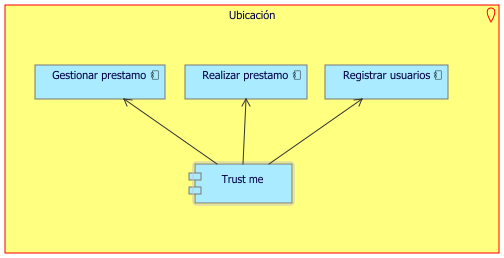
\includegraphics[width=0.7\linewidth]{development/cooperacionapp.pdf}
			\caption{Cooperación de Aplicación}
		\end{figure}
		\begin{center}
			\textbf{Fuente:} Propia.
		\end{center}
	}
	
	\subsection{Punto de vista de uso de aplicación}
	{Es utilizada para el diseño de la aplicación donde se identificaran los servicios que serán requeridos y estarán disponibles, por el proceso de negocio y otras aplicaciones \cite{archimate}.\\
		
		\textbf{Modelo}\\
		\begin{figure}[H]
			\centering
			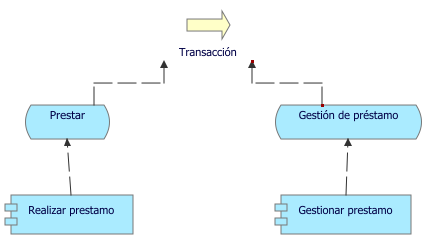
\includegraphics[width=0.7\linewidth]{development/usoapp.png}
			\caption{Metamodelo de Uso Aplicación}
		\end{figure}
		\begin{center}
			\textbf{Fuente:} Colosoft E.U: Documento CasoColoSoft.
		\end{center}
		
		\textbf{Caso:} Se presentan los principales servicios de la aplicación como lo son prestar y gestionar prestamos, los cuales son usados por los usuarios en el proceso del negocio.\\
		
		\begin{figure}[H]
			\centering
			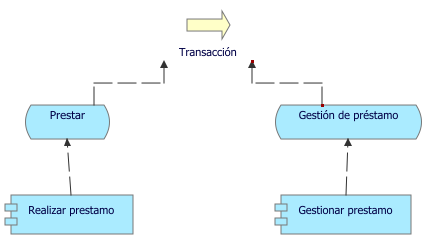
\includegraphics[width=0.8\linewidth]{development/usoapp.pdf}
			\caption{Uso Aplicación}
		\end{figure}
		\begin{center}
			\textbf{Fuente:} Propia.
		\end{center}
	}
	

			\section{Arquitectura capa de tecnología}

	\subsection{Punto de vista de infraestructura}
	{ 
		
		\textbf{Modelo}\\
		\begin{figure}[H]
			\centering
			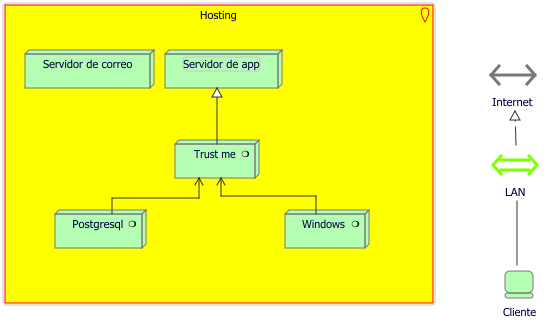
\includegraphics[width=0.8\linewidth]{development/infraestructura.png}
			\caption{Metamodelo de Infraestructura}
		\end{figure}
	
		\textbf{Caso:}
		
		\begin{figure}[H]
			\centering
			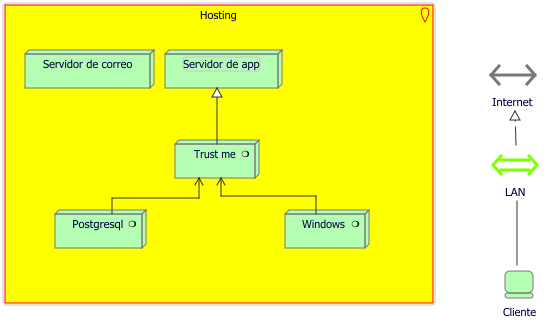
\includegraphics[width=0.6\linewidth]{development/infraestructura.pdf}
			\caption{Infraestructura}
		\end{figure}
	}
	
	\subsection{Punto de vista de uso de infraestructura}
	{
		
		\textbf{Modelo}\\
		\begin{figure}[H]
			\centering
			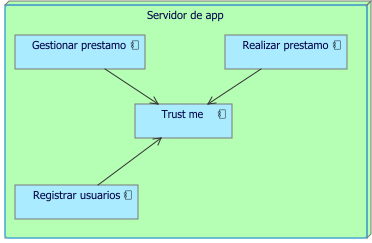
\includegraphics[width=0.8\linewidth]{development/usoinfraestructura.png}
			\caption{Metamodelo de Uso de Infraestructura}
		\end{figure}
		
		\textbf{Caso:} 
		
		\begin{figure}[H]
			\centering
			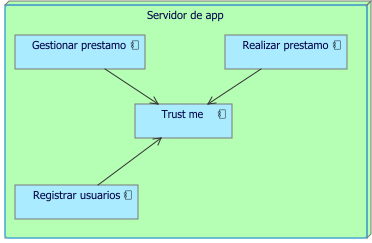
\includegraphics[width=0.8\linewidth]{development/usoinfraestructura.pdf}
			\caption{Uso de Infraestructura}
		\end{figure}
	}
	
	\subsection{Punto de vista de estructura de información}
	{		
		\textbf{Modelo}\\
		\begin{figure}[H]
			\centering
			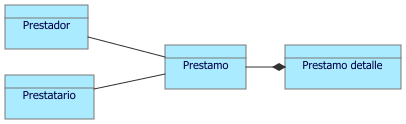
\includegraphics[width=0.8\linewidth]{development/estructurainfo.png}
			\caption{Metamodelo de Estructura de la información}
		\end{figure}
		
		\textbf{Caso:} 
		
		\begin{figure}[H]
			\centering
			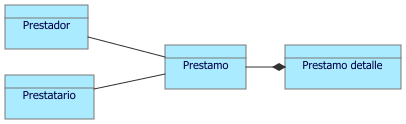
\includegraphics[width=0.8\linewidth]{development/estructurainfo.pdf}
			\caption{Estructura de la información}
		\end{figure}
	}
	
	\subsection{Punto de vista de realización del servicio}
	{ 		
		\textbf{Modelo}\\
		\begin{figure}[H]
			\centering
			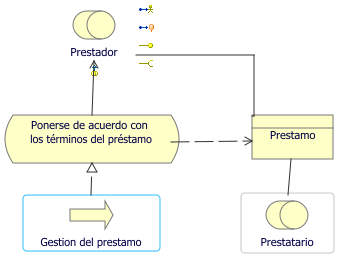
\includegraphics[width=0.8\linewidth]{development/realizacionser.png}
			\caption{Metamodelo de Realización Servicio}
		\end{figure}
		
		\textbf{Caso:}
			
		
		\begin{figure}[H]
			\centering
			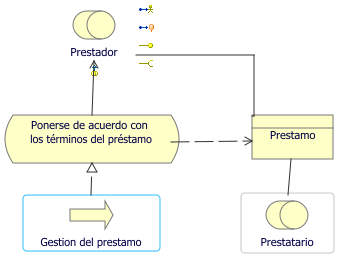
\includegraphics[width=0.8\linewidth]{development/realizacionser.pdf}
			\caption{Realización Servicio}
		\end{figure}
	}
	


	\part{CIERRE DE LA INVESTIGACIÓN}

		\chapter*{RESULTADOS Y DISCUSIÓN}
		\addcontentsline{toc}{chapter}{RESULTADOS Y DISCUSIÓN}
			\begin{itemize}
	\item Resultado 1.
	\item Resultado 2.
	\item Resultado 3.
\end{itemize}

		\chapter*{CONCLUSIONES}
		\addcontentsline{toc}{chapter}{CONCLUSIONES}
			Luego de haber finalizado el proyecto, se concluye lo siguiente:

\begin{itemize}
	
	\item El uso de la tecnología en el comercio y las estrategias de ventas como “fiar”, son unos pilares influyentes en el aumento de las ventas, pues estos permiten a sus consumidores acceder de forma fácil a sus productos y pagarlos cómodamente, generando satisfacción y fidelización en el cliente.
	
	\item Exponer de forma detallada y en tiempo real, las compras, deudas o transacciones realizadas entre el tendero y consumidor, genera un alto grado de confianza al usuario, ya que este, no estará con la incertidumbre referente a los pagos a realizar o ya realizados.
	
	\item Mostrar el monto total de las deudas y prestamos de los usuarios, es un mecanismo que ayuda autocontrolar a los mismos en cuanto a la adquisición de nuevas deudas se refiere, pues ellos sabrán lo máximo que pueden endeudarse y con base a eso, limitarse, de igual forma, ayuda a controlar el monto en prestamos a realizar, pues el usuario será consciente de lo máximo que le podrá prestar a otro.
	
\end{itemize}
			\section{Aportes Originales}

	\begin{itemize}
		
		\item Creación de un modelo empresarial donde se gestione los prestamos de los tenderos hacia sus consumidores.
		
		\item Permitir el acceso de personas de bajos recursos a productos de bajo costo, por medio de la tecnología.
		
		\item Procesar las apuestas informales o deudas entre conocidos, para tener un mejor control de estas.
		
	\end{itemize}
			\section{Trabajos o publicaciones derivadas}
	{El modelo de negocio planteado, puede derivar en la creación propia de cada tendero de su sitio WEB, donde procese los pagos de sus clientes y obtener un control o dominio total, de lo que se acontece en su negocio.}
			
		\chapter*{PROSPECTIVA DEL TRABAJO DE GRADO}
		\addcontentsline{toc}{chapter}{PROSPECTIVA DEL TRABAJO DE GRADO}
			\section{Trabajos de investigación futuros}

	{A futuro, se propone implementar lo siguiente:
		
	\begin{itemize}
		\item Una integración con centros de pagos, que permitan procesar el pago online de sus deudas con sus respectivos prestamistas y así, evitar el manejo de efectivo, acercando un poco más la plataforma a las últimas tendencias tecnológicas de los usuarios.
		
		\item Una arquitectura de software mantenible y desacoplada por medio de microservicios, que permita la integración vía API con varias tecnologías, como lo es Android, IPhone, Mac, Windows etc. Posibilitando el renderizado de vistas según la información suministrada por el microservicio, utilizando cualquier lenguaje de programación.
	\end{itemize}
		
	Por otro lado, se pretende ampliar el modelo de negocio propuesto, donde se permita abarcar almacenes de cadena que accedan a este tipo de actividad económica, posibilitando un ingreso económico extra.
	}
\clearpage
			
	\renewcommand{\bibname}{REFERENCIAS}	
	\bibliographystyle{ieeetr}
	\addcontentsline{toc}{part}{REFERENCIAS}
	\bibliography{bibliography/articles,bibliography/books,bibliography/online}
	
	\chapter*{ANEXOS}
	\addcontentsline{toc}{part}{ANEXOS}
		\section*{Anexo A. Recolección de la información}
\addcontentsline{toc}{section}{Anexo A. Recolección de la información}

	\subsection*{Encuesta}
	\addcontentsline{toc}{subsection}{Encuesta}
	
	{Para obtener la información base para el desarrollo del proyecto, fue indispensable utilizar la técnica de recolección de información “encuesta”, donde se plasmaron las inquietudes que permitieron estructurar adecuadamente el proyecto.\\
		
	Las encuestas realizadas fueron las siguientes (se utilizó la plataforma Formularios de Google para publicar y obtener los resultados de estas):
	
	
		\subsubsection*{Encuesta 1 - Viabilidad}
		\addcontentsline{toc}{subsubsection}{Encuesta 1 - Viabilidad}
		
			\begin{enumerate}
				
				\item ¿Ha recurrido el sistema de “fiado” que utilizan algunos tenderos para adquirir productos?
				
					\begin{enumerate}
						\item Si.
						\item No.
					\end{enumerate}
				
				\item ¿Ha tenido problemas al momento de pagar sus productos fiados, ya que el monto de la deuda es mayor o menor al que tenía en mente?
				
					\begin{enumerate}
						\item Si.
						\item No.
					\end{enumerate}	
				
				\item Cuándo realiza un préstamo, ¿dónde realiza el registro de este, para su posterior control?
					
					\begin{enumerate}
						\item Tomo notas en el celular.
						\item Tomo notas en cuadernos o agendas.
						\item No tomo notas.
						\item Otro.
					\end{enumerate}
				
				\item ¿Suele olvidarse de las deudas que tienen algunas personas con usted (personas de confianza)?
				
					\begin{enumerate}
						\item Si.
						\item No.
					\end{enumerate}	
				
				\item Considera que utilizar una plataforma Web que permita gestionar los fiados y prestamos es:
				
					\begin{enumerate}
						\item Pertinente.
						\item Innecesaria.
					\end{enumerate}
				
			\end{enumerate}
		
		\subsubsection*{Tabulación encuesta 1}
		\addcontentsline{toc}{subsubsection}{Tabulación encuesta 1}
		{Para esta encuesta, se alcanzaron a encuestar 71 personas que contestaron lo siguiente:
		
		\begin{figure}[H]
			\centering
			\includegraphics[width=0.8\linewidth]{annexes/e1-p1.png}
			\caption{Diagrama de torta E-1 P-1}
		\end{figure}
	
		\begin{figure}[H]
			\centering
			\includegraphics[width=0.8\linewidth]{annexes/e1-p2.png}
			\caption{Diagrama de torta E-1 P-2}
		\end{figure}
	
		\begin{figure}[H]
			\centering
			\includegraphics[width=0.8\linewidth]{annexes/e1-p3.png}
			\caption{Diagrama de torta E-1 P-3}
		\end{figure}
	
		\begin{figure}[H]
			\centering
			\includegraphics[width=0.8\linewidth]{annexes/e1-p4.png}
			\caption{Diagrama de torta E-1 P-4}
		\end{figure}
	
		\begin{figure}[H]
			\centering
			\includegraphics[width=0.8\linewidth]{annexes/e1-p5.png}
			\caption{Diagrama de torta E-1 P-5}
		\end{figure}
		}
		
		\subsubsection*{Encuesta 2 - Satisfacción del proyecto}
		\addcontentsline{toc}{subsubsection}{Encuesta 2 - Satisfacción del proyecto}
		
			\begin{enumerate}
				
				\item Utilizando Tru\$tMe como tendero sus ventas han:
				
				\begin{enumerate}
					\item Aumentado.
					\item Se mantuvieron.
					\item Disminuido.
				\end{enumerate}
				
				\item Utilizando Tru\$tMe como consumidor, ¿Ha tenido dudas con respecto a los pagos a realizar?
				
				\begin{enumerate}
					\item Si.
					\item No.
				\end{enumerate}	
				
				\item ¿Le permite Tru\$tMe tener un mejor control de sus finanzas visualizando sus deudas y prestamos actuales?
				
				\begin{enumerate}
					\item Si.
					\item No.
				\end{enumerate}
				
			\end{enumerate}
		
		\subsubsection*{Tabulación encuesta 2}
		\addcontentsline{toc}{subsubsection}{Tabulación encuesta 2}
		
		{Para esta encuesta, se alcanzaron a encuestar 23 personas que contestaron lo siguiente:
			
			\begin{figure}[H]
				\centering
				\includegraphics[width=0.8\linewidth]{annexes/e2-p1.png}
				\caption{Diagrama de torta E-2 P-1}
			\end{figure}
			
			\begin{figure}[H]
				\centering
				\includegraphics[width=0.8\linewidth]{annexes/e2-p2.png}
				\caption{Diagrama de torta E-2 P-2}
			\end{figure}
			
			\begin{figure}[H]
				\centering
				\includegraphics[width=0.8\linewidth]{annexes/e2-p3.png}
				\caption{Diagrama de torta E-2 P-3}
			\end{figure}
		}
		
	}
	

	
	

\end{document}          
